\subsection{Amélioration de la rétropropagation}



\begin{frame}{La quantité de mouvement (momentum)}
    \begin{block}{Descente de gradient avec momentum}
        $x_0$ aléatoire, momentum $\omega_0 = 0$.
        $x_0, \ldots, x_k$ et $\omega_0, \ldots, \omega_k$ construits. \\
        • On pose $\omega_{k+1} = \gamma \omega_k + t \nabla f(x_k)$ \\
        • On pose $x_{k+1} = x_k - \omega_{k+1}$
    \end{block}
    \begin{figure}
        \centering
        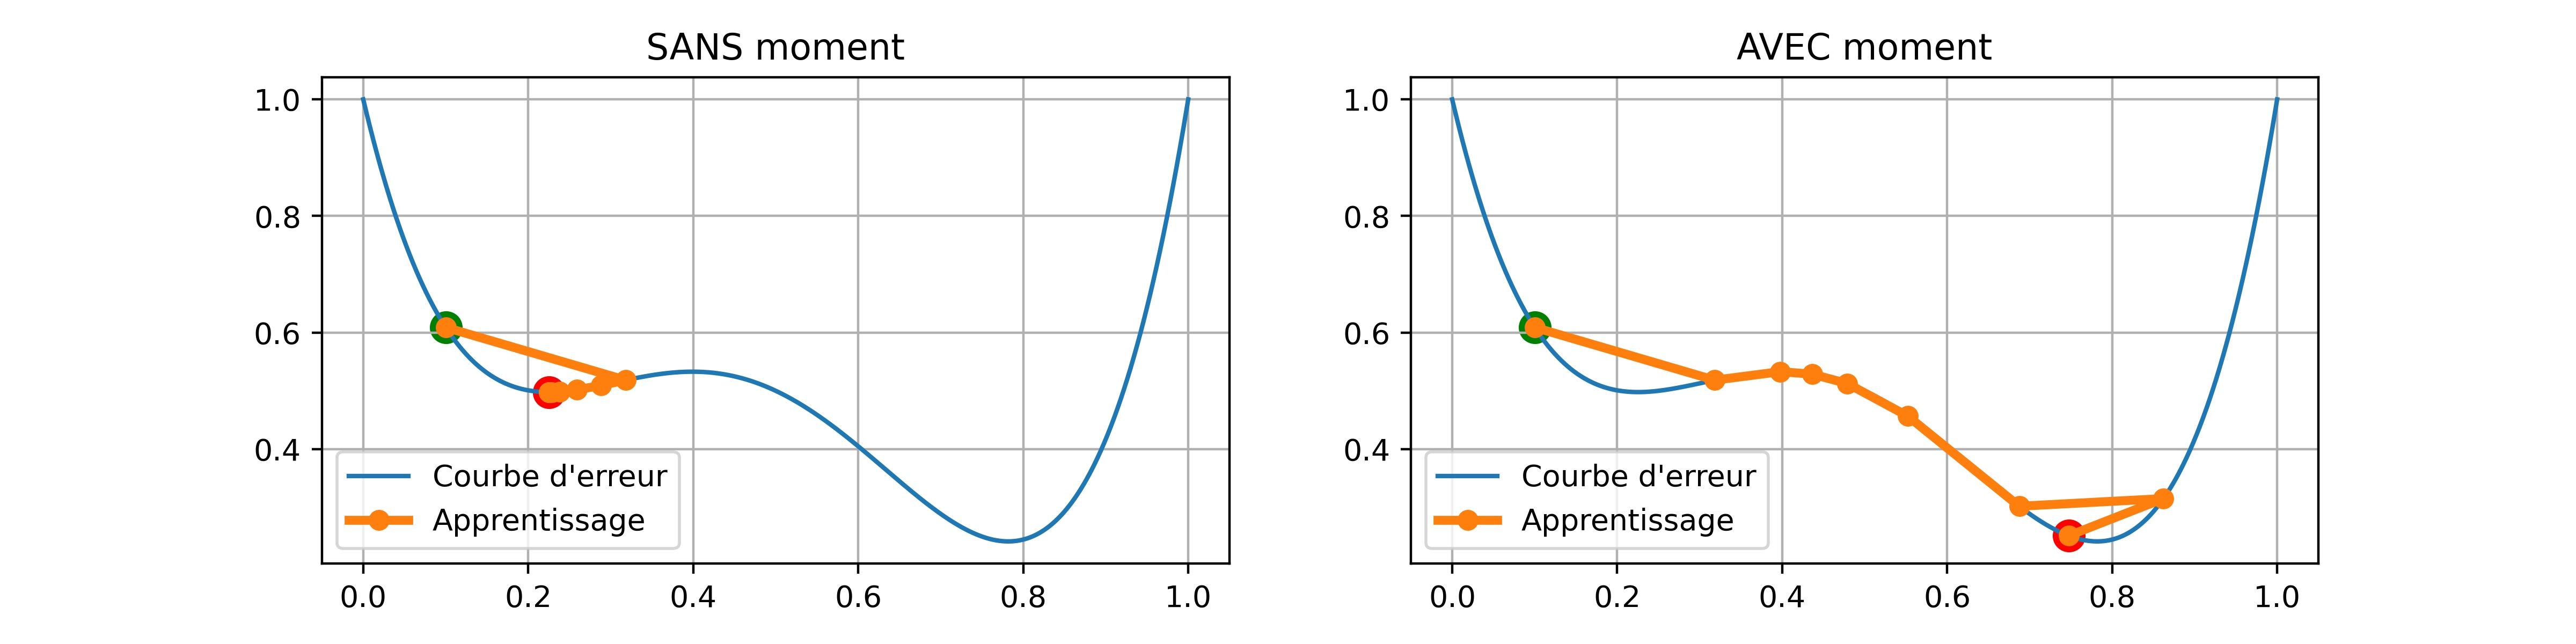
\includegraphics[height=120px]{4-Moment.jpg}
        \caption{Descente de gradient SANS/AVEC momentum où $\gamma = 0.5$}
    \end{figure}
\end{frame}



\begin{frame}{Les avantages du momentum}
    \begin{exampleblock}{Avantages}
        \begin{itemize}
            \item La descente de gradient converge lentement
            \item La descente de gradient s'échappe de minima locaux  
        \end{itemize}  
    \end{exampleblock}
    \begin{figure}
        \centering
        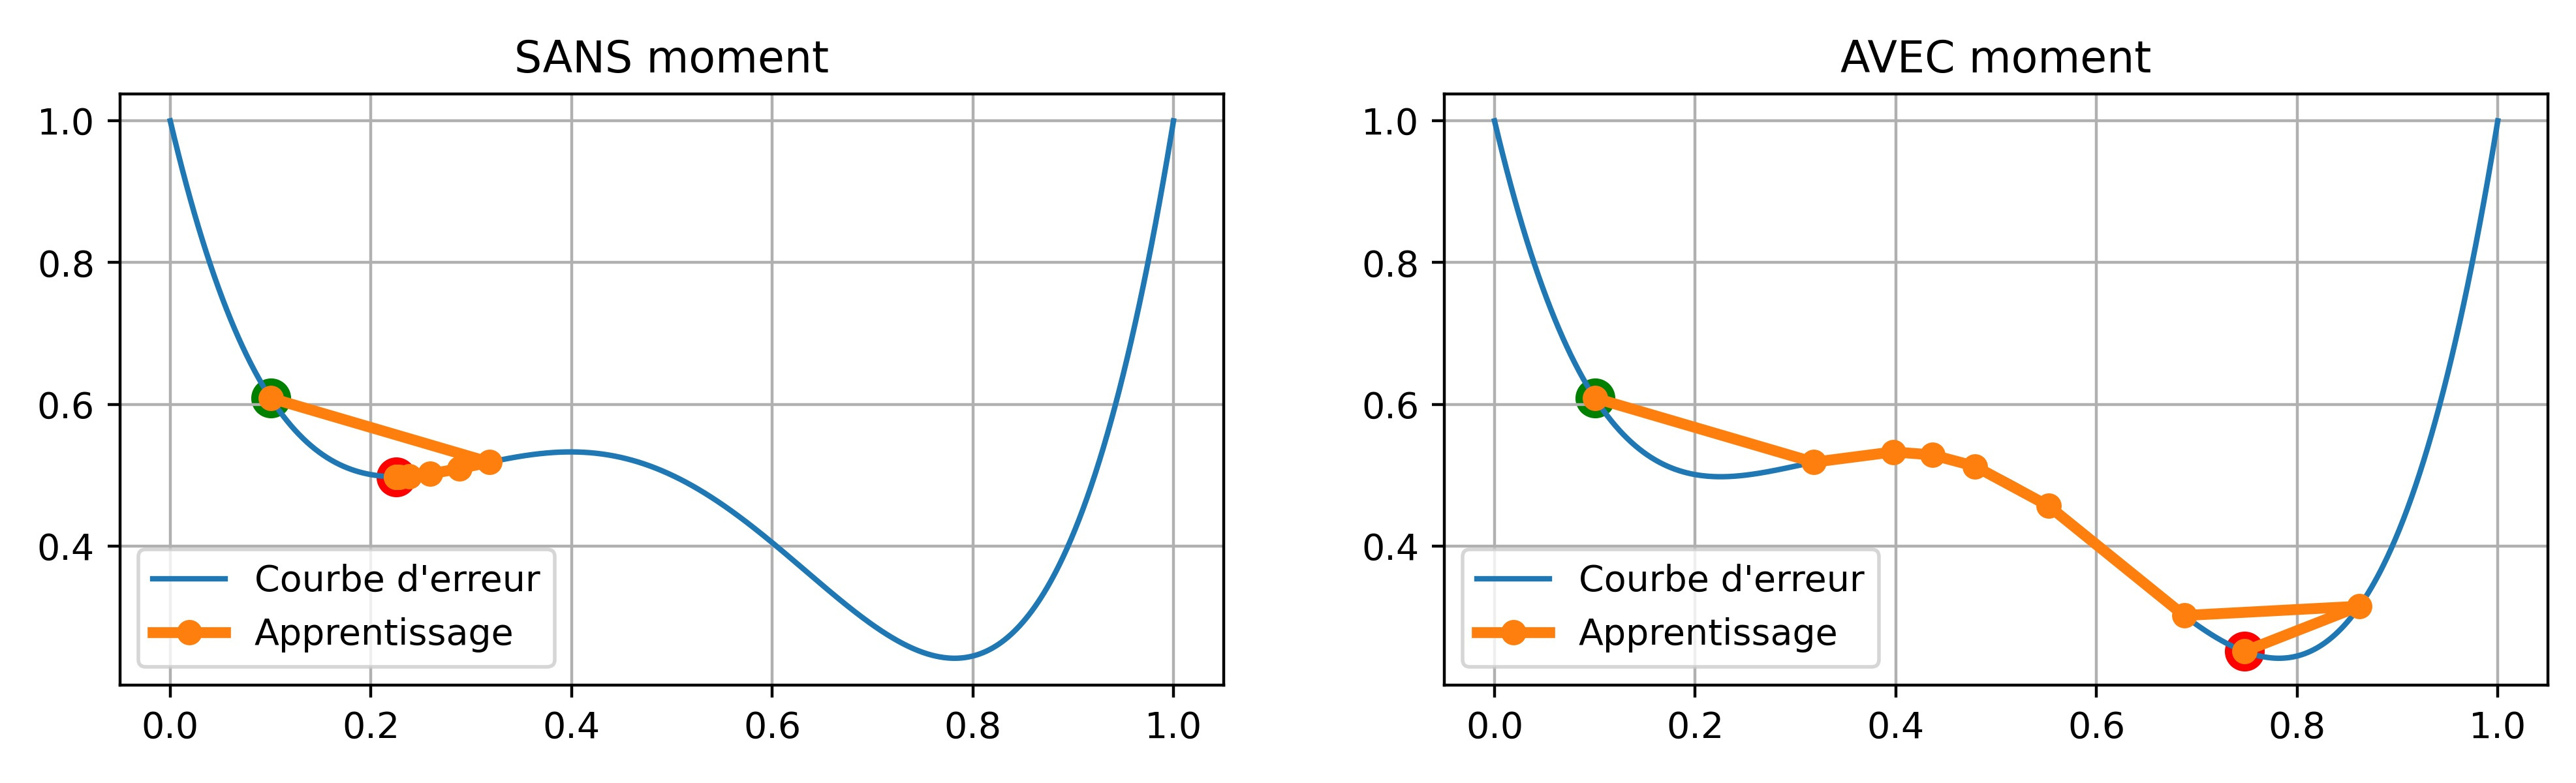
\includegraphics[width=\textwidth]{5-Moment.jpg}
        \caption{Descente de gradient SANS/AVEC momentum où $\gamma = 0.5$}
    \end{figure}
\end{frame}




\begin{frame}{L'apprentissage stochastique ou par paquet (batch)}
    \begin{alertblock}{Problème d'incertitude des données}
        Les données d'apprentissage ne sont pas toujours exactes. \\
        J'ajoute donc aux données théoriques de mon test une valeur d'incertitude, pour se rapprocher au plus de la réalité. 
    \end{alertblock}
    \begin{exampleblock}{Solution}
        Il est alors préférable d'appliquer la rétropropagation à notre réseau sur des paquets de données plutôt que donnée par donnée. 
    \end{exampleblock}
    \begin{center}
        \centering
        $
            \left< f
            \left(
            \begin{pmatrix}
                    x_1^{1} & \ldots & x_n^{1} & b      \\
                    \vdots  & \vdots & \vdots  & \vdots \\
                    x_1^{D} & \ldots & x_n^{D} & b
                \end{pmatrix}
            \times
            \begin{pmatrix}
                    w_1    \\
                    \vdots \\
                    w_n    \\
                    w_b
                \end{pmatrix}
            \right) \right>
        $
    \end{center}
\end{frame}


\begin{frame}{Une illustration de l'apprentissage par batch}
    \begin{figure}
        \centering
        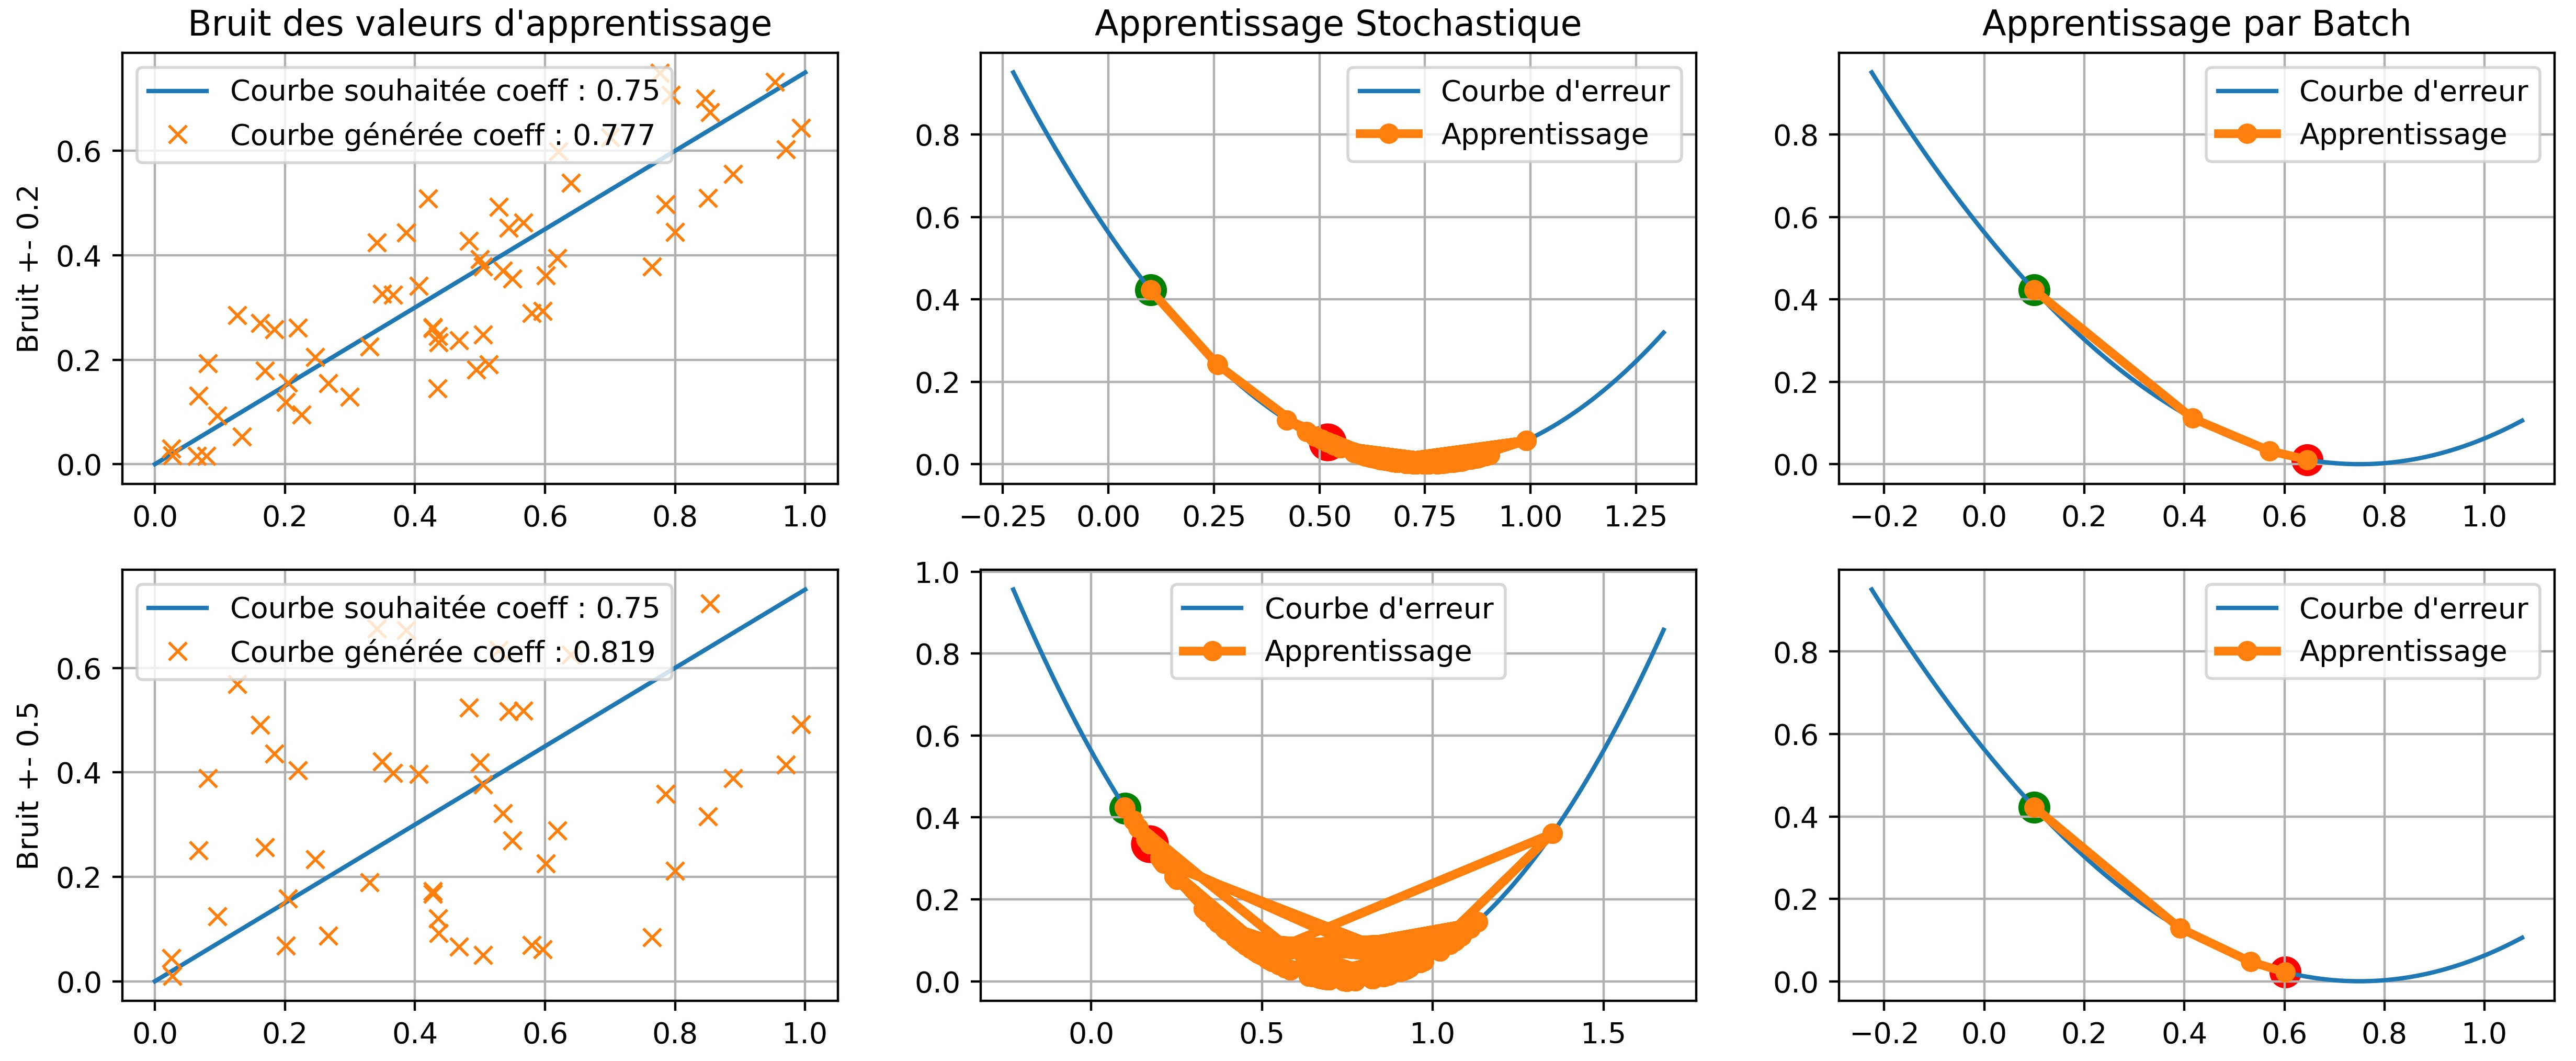
\includegraphics[width=\textwidth]{7-Batch.jpg}
        \caption{Comparaison apprentissage stochastique et par paquet}
    \end{figure}
\end{frame}
